
\setcounter{page}{53}
\setlength{\parskip}{0em}
\setlength{\parindent}{2em}
\setstretch{0.9}


\begin{multicols}{2} % начало двух колонок

\noindent ках — языках программирования. С грамматикой некоторых языков (Рапиры, Паскаля) вы уже, наверное, знакомы, ну а какие обороты в каких случаях надо применять? Вот на этот вопрос, а заодно и на вопрос, как понимает ЭВМ неправильные обороты, мы и попытаемся дать ответ.

\section*{\normalsize Подготовительные задачи к уроку 1}

	\begin{enumerate}[label=\bfseries\arabic*., wide=0pt,itemindent = 2em]
		\item Дано число $x$. Вычислить приближенное значение $\sqrt{x}$ с точностью $\varepsilon$ с помощью метода последовательных приближений:
		\[
			y_0 = \frac{x}{2}, \quad y_i = \frac{1}{2} \left( y_{i-1} + \frac{x}{y_{i-1}} \right), \quad i \ge 1
		\]
		Вычисления вести до тех пор, пока не станет \linebreak$|y_i - y_{i-1}| < e$.
		
		\item Напечатать значения первых \textit{N} чисел Фибоначчи\footnote[1]{Об этих замечательных числах можно прочитать в «Кванте» 1979, №5, с. 53 или в брошюре Н. Н. \so{Воробьёва} «Числа Фибоначчи» (М., «Наука», 1978), но для решения задачи это требуется}\linebreak  
		$f_0 = 1$, $f_1 = 1$, $f_i = f_{i-1} + f_{i-2}$, $i \ge 2$.
		
		\item Даны массив коэффициентов $a_i$, $i = 0, \dots, n$, и значение $x$. Вычислить значение многочлена
			\[
				y = \sum_{i=0}^{n} a_i x^i  \;\text{применяя формулу:}
			\]
			\[
				y = (\dots(a_n x + a_{n-1})x + \dots\vphantom  ++ a_1)x + a_0
			\]
		(Этот очень эффективный прием вычисления многочленов называется \textit{схемой Горнера}: в нем $n$ сложений, $n$ умножения и ни одного (!) возведения в степень.)
		
		\item Дано $x$. Вычислить приближенное значение $\sin x$ с точностью $\varepsilon$, пользуясь формулой  
			\[
				\sin x \approx x - \frac{x^3}{3!} + \frac{x^5}{5!} - \frac{x^7}{7!} + \dots\vphantom  ++ (-1)^n \frac{x^{2n+1}}{(2n+1)!}
			\]
		Считать известным, что точность $\varepsilon$ будет достигнута, когда  
			\[
				\left| \frac{x^{2n+1}}{(2n+1)!} \right| < \varepsilon.
			\]
		
	\end{enumerate}

\indent В задачах 1, 2 не использовать массивы. В задаче 4 не использовать возведение в степень.

\vspace{1em}

\indent После решения задач внимательно сравните условия и решения всех задач, и попробуйте ответить на вопросы:


	\begin{enumerate}[itemindent = 1em,label=\arabic*)]
		\item что общего в условиях этих задач?
		\item что общего в их решениях?
	\end{enumerate}

\indent Сравните ваши решения с приведенными на с. 54. Задача 3, наверное, трудностей не вызвала. Если в задачах 1, 2, 4 ваши решения построены на тех же идеях, что и решения а), то вы сделали все правильно, а если на идеях решений б), то вы ошиблись. Конечно, и программы б) будут работать и дадут в большинстве случаев нужный вам результат, и все же любой опытный программист скажет, что они не годятся. Почему?

\indent Для ответа на этот вопрос давайте посмотрим, что общего в условиях и решениях задач. Вы заметили, наверное, и часто пользоваться определенными операциями и переприсваивания значений (обведены рамочкой). \columnbreak 

Но самым главным является то, что \textbf{очередные значения вычисляются через предыдущие} (см. подчеркнутые части программ). В математике зависимость новых значений от старых называется \textit{рекуррентной}, а число старых значений, от которых зависит очередное значение, называется \textit{порядком} рекуррентной формулы.

\indent Таким образом, в задачах 1 и 2 мы \so{имели} рекуррентные формулы соответственно 1-го и 2-го порядка, а в задачах 3 и 4 мы \so{свели} неперекуррентную запись многочлена и формулы (1) к рекуррентной:
	\[
		y = \sum_{i=0}^{n} a_i x^i \Rightarrow y_0 = a_n, \quad y_i = y_{i-1} x + a_{n-i}
	\]
	\[
		y = \sum_{i=0}^{n} (-1)^i \frac{x^{2i+1}}{(2i + 1)!} \Rightarrow y_0 = 0, 
	\]
	\[
		\quad z_0 = x; \quad y_i = y_{i-1} + z_{i-1}; \quad z_i = \frac{-z_{i-1}x^2}{2i(2i + 1)}.
	\]
\vspace{1em}

\indent Теперь взглянем на решения б) и зададим себе вопрос: если бы вы вручную считали по формуле (1), то разве стали бы вы вычислять каждый раз степень или считать факториал заново? Вряд ли. А потому нужно использовать рекуррентные варианты, а это значит, что нужно хранить промежуточные значения. А в задаче 1 и вообще неясно, сколько этих промежуточных значений будет и какой объем памяти под них надо отвести. Кроме того, оказывается, что для ЭВМ операции индексирования — это очень трудоемкая операция: более трудоемкая, чем, например, умножение (вообще «точка зрения» ЭВМ на трудоемкость отдельных операций совсем не совпадает с человеческой). Теперь вам стали ясны запреты в условиях задач: мы запретили лишний раз расходовать память и использовать трудоемкие операции. Современные ЭВМ имеют огромную память и колоссальную скорость, и все же есть очень много задач, для которых скорости и памяти не хватает. Поэтому программист должен уметь бережно расходовать ресурсы ЭВМ и, следовательно, решения б) нельзя признать пригодными.

\indent Откуда же появляются такие ошибки? Дело в том, что программист часто переводит алгоритм с языка математики на язык программирования. Эти языки похожи, но правила «разговора» на них различны. Поэтому «подстрочный» перевод с языка математики на язык программирования может дать совсем неправильный результат, также как дословный перевод русского приветствия «Добрый день!» на английский — «Kind day!» — ошибочен: для англичанина это не приветствие, а бессмыслица.

\indent Возвращаясь к нашим задачам, отметим разницу в «правилах разговора» на языке математики и языке программирования. \textit{Математики используют индексацию для различных значений переменных как «в пространстве», так и «во времени», программисты — только для различения в пространстве}. В рекуррентных формулах индексы характеризуют время (номер шага) появления очередного значения, поэтому при программировании 
они не нужны: новые значения просто засылаются на старое место.

\vfill
\end{multicols} % конец двух колонок

\clearpage
\setcounter{page}{54}
\setstretch{0.9}
\setlength{\tabcolsep}{10pt} % Горизонтальные отступы слева/справа
\renewcommand{\arraystretch}{1.5} % Вертикальные отступы

\centering
\section*{Решения подготовительных задач к уроку 1}

\begin{tabular}{|p{0.45\textwidth}|p{0.48\textwidth}|}
	 \hline
	 \multicolumn{2}{|c|}{(Описания и ввод-вывод опущены, приведены только тела программ) } \\
	 \multicolumn{2}{|c|}{(a)\hspace{8.4cm}(б)} \\
	 \hline
	 \multicolumn{2}{|l|}{\small\textbf{Задача 1} (Квадратный корень)} \\
	 \hline
		 \begin{minipage}{0.46\textwidth}
			 \small
			 \texttt{\\y := x/2;}\\[1pt]
			 \texttt{\textbf{repeat}\quad \boxed{\texttt{y0 := y;}}}\\[1pt]
			 \texttt{y := 0.5 * (y0 + x/y0)}\\[-1.5pt]
			 \texttt{\textbf{until} \textit{abs}(y0 - y1) < \textit{eps};}\\[-1.5pt]
		 \end{minipage}
	 &
		 \begin{minipage}{0.46\textwidth}
			 \small
			 \texttt{\\y[0] := x/2; i := 0;}\\[-1.5pt]
			 \texttt{\textbf{repeat} \quad i := i + 1;}\\[-0.5pt]
			 \texttt{\phantom{a}\quad y[i] := 0.5 * (y[i-1] + x/y[i-1])}\\[-0.5pt]
			 \texttt{\textbf{until} \textit{abs}(y[i] - y[i-1]) < \textit{eps};}\\[-1.5pt]
		 \end{minipage} \\ 
	 \hline
	 \multicolumn{2}{|l|}{\small\textbf{Задача 2} (Числа Фибоначчи)} \\
	 \hline
		 \begin{minipage}{0.46\textwidth}
			 \small
			 \texttt{\\f2 := 1; f1 := 1;}\\[-1.5pt]
			 \texttt{for i := 3 to \textit{n} do}\\[-1.5pt]
			 \texttt{begin\quad f := f2 + f1:\quad \textit{writeln(f)};}\\[1pt]
			 \texttt{\phantom{a}\: \boxed{\texttt{f2 := f1:\quad f1 := f}}}\\[1pt]
			 \texttt{end;}\\[-1.5pt]
		 \end{minipage}
	 &
		 \begin{minipage}{0.46\textwidth}
			 \small
			 \texttt{\\f[$\varnothing$] := 1; f[1] := 1;}\\[-1.5pt]
			 \texttt{\textbf{for} i := 3 to \textit{n} do}\\[-1.5pt]
			 \texttt{begin\quad f[i] := f[i-1] + f[i-2];}\\[-1.5pt]
			 \texttt{\phantom{a} \quad \textit{writeln(f[i])}}\\[-1.5pt]
			 \texttt{end;}\\[-1.5pt]
		 \end{minipage} \\ 
	 \hline
	 \multicolumn{2}{|l|}{\small\textbf{Задача 3} (Схема Горнера)} \\
	 \hline
		 \begin{minipage}{0.46\textwidth}
			 \small
			 \texttt{\\y := a[n];}\\[-1pt]
			 \texttt{for i := n-1 downto 0 do}\\[-1pt]
			 \texttt{\phantom{a} \quad y := y * x + a[i];}\\[-1pt]
		 \end{minipage}
	 & 
		 \begin{minipage}{0.46\textwidth}
			 % Пустая ячейка для (б)
		 \end{minipage} \\
	 \hline
	 \multicolumn{2}{|l|}{\small\textbf{Задача 4} (Вычисление синуса)} \\
	 \hline
		 \begin{minipage}{0.46\textwidth}
			 \small
			 \texttt{\\s := 0; \textit{элем} := x; k := 1;}\\[-1.5pt]
			 \texttt{while \textit{abs}(\textit{элем}) > \textit{eps} do}\\[-1.5pt]
			 \texttt{begin \quad s := s + \textit{элем}; k := k + 2;}\\[-1.5pt]
			 \texttt{\phantom{a}\quad \textit{элем} := -\textit{элем} * x * x / (k * (k-1))}\\[-1.5pt]
			 \texttt{end;}\\[-1.5pt]
		 \end{minipage}
	 &
		 \begin{minipage}{0.46\textwidth}
			 \small
			 \texttt{\\s := 0; \textit{элем} := x; k := 0;}\\[-1.5pt]
			 \texttt{while \textit{abs}(\textit{элем}) > \textit{eps} do}\\[-1.5pt]
			 \texttt{begin\quad s := s + \textit{элем}; k := k + 1;}\\[-1.5pt]
			 \texttt{\phantom{a}\quad \textit{факт} := 1;}\\[-1.5pt]
			 \texttt{\phantom{a}\quad for i := 2 to 2*k+1 do \textit{факт} := \textit{факт} * i;}\\[-1.5pt]
			 \texttt{\phantom{a}\quad \textit{факт} := \textit{степ}(-1,k) * \textit{степ}(x,2*k+1) / \textit{факт}}\\[0.5pt]
			\texttt{\{функция \textit{степ}(a,n) даёт значение $\textit{a}^\textit{n}$ \}}\\
			 \texttt{end;}\\
		 \end{minipage} \\
	 \hline
	\end{tabular}
\newline

\justifying
\noindent \newline Таким образом:
\begin{multicols}{2} 

	\hspace{2em}\begin{minipage}{0.8\linewidth}
		\hspace{2em}\small\textbf{При счете по рекуррентной формуле $k$-го порядка достаточно иметь $k+1$ дополнительный элемент памяти для хранения последних $k$ значений и очередного значения.}
	\end{minipage}
\\ \\ \\
\indent В рекуррентных формулах $1$-го порядка, если не надо сравнивать соседние значения, можно обойтись вообще одним элементом (см. задачу 3).

\hspace{2em} Программы, реализующие рекуррентные соотношения, включают в себя следующие фрагменты:
	\begin{enumerate}[label=—,wide=0pt,itemindent = 2em]
		\item начальные присваивания (в решениях — это первые строчки)
		\item основной цикл счета по формулам, 
		\item в теле цикла: вычисление очередного значения, использование этого значения и переприсваивание 
	\end{enumerate} 
\hspace{2em} Эти элементы имеются обязательно, хотя выглядеть могут по-разному. Начальные присваивания могут выполняться по сложному алгоритму. Основной цикл может быть с заранее известным (как в задачах 2, 3) или заранее неизвестным числом повторений (как в задачах 1, 4). В формулах 1-го порядка переписывание может быть совмещено с вычислением очередного значения. Очередное значение может использоваться в дальнейших расчетах (как значение \textit{элем} в задаче 4), просто печататься (задача 2) или не использовать вообще для чего-либо иного, кроме получения следующего значения.

\hspace{2em} В заключение рассмотрим задачу с рекуррентной формулой \textit{$k$-го порядка: напечатать первые $N$ значений, определяемых рекуррентными формулами:}\\

$f_i = 1, \: f \le k; \: f_{i+1} = (f_{i-k+1} + f_{i-k+2} + \dots\vphantom + + f_{i-1})f_i. $\\[-6pt]

\centering
$i \ge k$ \\[8pt]
\justifying
\hspace{2em} Для решения нам понадобится массив в $k+1$ элемент для размещения последних $k$ значений и нового значения. Обратите внимание: этот массив работает как трамвай: очередное значение «входит» в него через переднюю дверь (а не в заднюю, как мы привыкли), «проезжает» \textit{$k$ остановок, проваливаясь назад,}

\hspace{1em}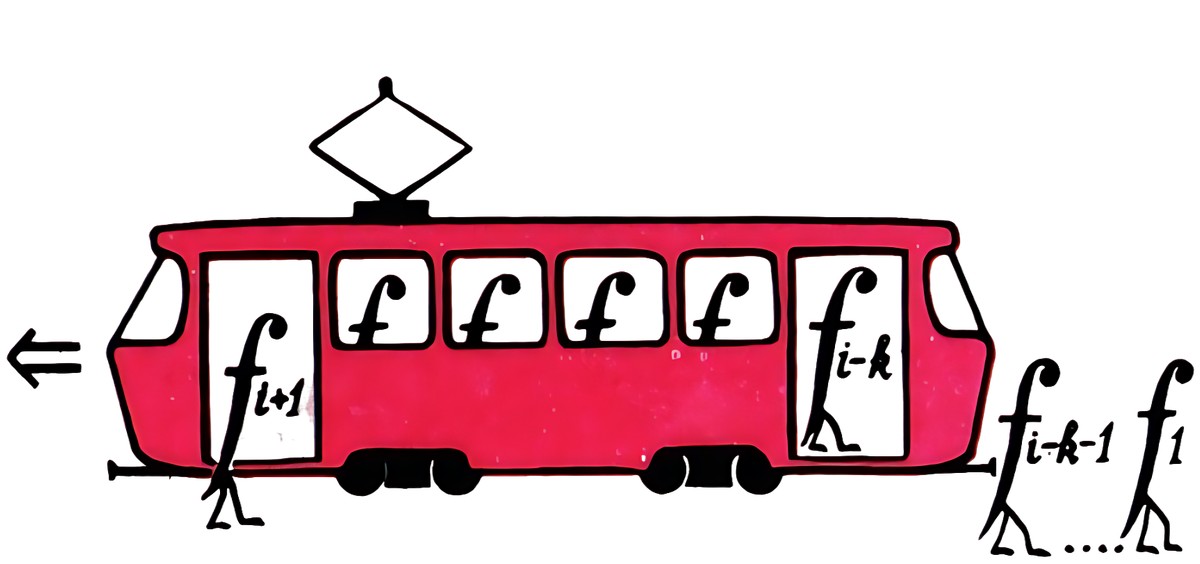
\includegraphics[scale=0.3, angle=-0.5]{images/photo.png}
\end{multicols}